
%(BEGIN_QUESTION)
% Copyright 2008, Tony R. Kuphaldt, released under the Creative Commons Attribution License (v 1.0)
% This means you may do almost anything with this work of mine, so long as you give me proper credit

Examine this process trend, showing the response of the process variable to a 50\% step change in the controller setpoint (placed in automatic mode).  This is a P+I controller (no derivative), and the output trend is not shown:

$$\includegraphics[width=15.5cm]{i03401x01.eps}$$

Note how the process variable oscillates on its way up to the new setpoint value.  This oscillatory motion {\it prior} to achieving setpoint (sometimes referred to by the charming term of ``porpoising'') is definitely the result of excessive proportional action and cannot be the result of integral action.

Explain how we can know this with confidence.  How is it possible to tell, just from viewing the ``porpoising'' action of the process variable, that the controller has too much gain rather than too much reset?  Expressed another way, how can we know with certainty that integral action is not responsible for the porpoising?

\vskip 20pt \vbox{\hrule \hbox{\strut \vrule{} {\bf Suggestions for Socratic discussion} \vrule} \hrule}

\begin{itemize}
\item{} What's wrong with porpoising anyway, so long as the PV never overshoots SP?
\item{} How {\it would} a process variable oscillate if it were the integral action of the controller tuned too aggressively?
\item{} Is there any way to tell from an examination of the closed-loop trend whether the cause of the porpoising is proportional action or derivative action?
\end{itemize}

\underbar{file i03401}
%(END_QUESTION)





%(BEGIN_ANSWER)

Oscillation in the process variable is the result of the controller's output (valve position) reversing direction.  Integral action {\it cannot} reverse valve direction so long as the error remains the same sign (either positive or negative).  Therefore, the only actions capable of reversing valve direction prior to achieving setpoint are proportional and derivative.  Since we know this particular controller has no derivative action, the excess must be proportional (i.e. too much gain).

%(END_ANSWER)





%(BEGIN_NOTES)

If we were to add an Output (PD) trend to the graph and examine the phase shift between PV and Output waveforms, it would clearly indicate whether proportional action or derivative action was to blame.  P action would exhibit very little phase shift, while D action would exhibit a leading phase shift (close to +90$^{o}$).






\vfil \eject

\noindent
{\bf Prep Quiz:}

Suppose a full PID controller exhibits the following response following a setpoint step-change.  Identify the actions capable of causing this ``porpoising'':

$$\includegraphics[width=15.5cm]{i03401x01.eps}$$

\begin{itemize}
\item{} Integral action or derivative action
\vskip 5pt 
\item{} Proportional action or integral action
\vskip 5pt 
\item{} Only integral action can do this
\vskip 5pt 
\item{} Only derivative action can do this
\vskip 5pt 
\item{} Proportional action or derivative action
\vskip 5pt 
\item{} Only proportional action can do this
\end{itemize}


%INDEX% Control, PID tuning: porpoising
%INDEX% Control, PID tuning: process responses to excessive proportional action

%(END_NOTES)


